Una vez presentado el contexto, los objetivos, así como las herramientas empleadas, en este capítulo se detalla la mejora desarrollada sobre la herramienta Scratch4Robots. Primero presentamos el diseño global y después analizaremos en detalle que aportaciones se han realizado y como se han llevado a cabo. Este apartado nos ayudará a entender en profundidad y el alcance de las mejoras realizadas sobre Scratch4Robots 1.0.\\

\clearpage
\section{Diseño}
\label{sec:diseno}
Como diseño global de la herramienta, y detallando poco el funcionamiento su funcionamiento interno, podemos esquematizar Scratch4Robots 2.0 de la siguiente forma:\\

\begin{figure}[H]
    \centering
    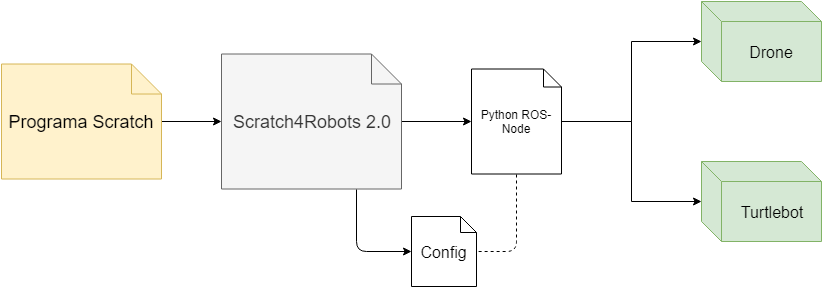
\includegraphics[scale=0.55]{img/esq-caja-negra.png}
  	\caption{Esquema de Scratach4Robots 2.0}
  	\label{fig:s4r-detalle}
\end{figure}

Esta es la poca complejidad con la que el usuario final tiene que lidiar, apreciándose su sencillez en el diseño y entendimiento a simple vista.\\

El diseño básico consta de un programa, codificado mediante el lenguaje visual Scratch 2.0, que nuestra herramienta, Scratch4Robots 2.0, procesará y traducirá. Como resultado de este proceso obtenemos un nodo ROS, programado en Python, y un fichero de configuración, necesario para su ejecución. Este nodo ya estará preparado para ser ejecutado sobre drones y robots Turtlebots.\\

Después de ver el diseño superficial, vamos a detallar como funciona de forma interna Scratch4Robots 2.0. En el siguiente esquema podemos apreciar los componentes internos en los que se basa la herramienta.\\

\begin{figure}[H]
    \centering
    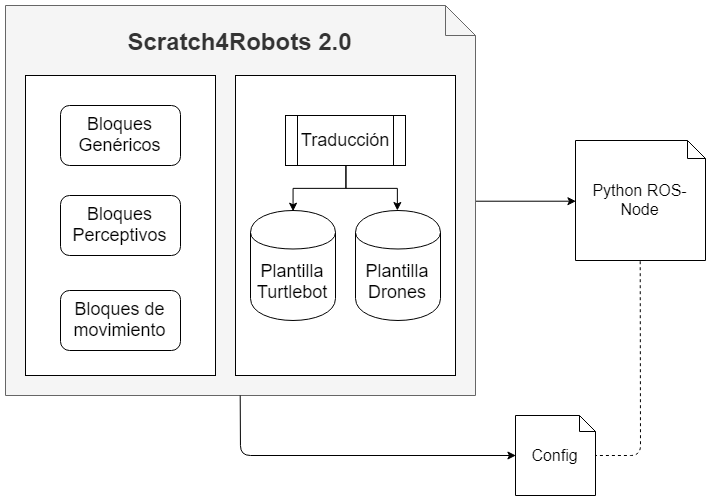
\includegraphics[scale=0.55]{img/esq-caja-blanca.png}
  	\caption{Esquema de Scratch4Robots 2.0 en detalle}
  	\label{fig:s4r}
\end{figure}

En un primer apartado podemos ver los bloques visuales que soporta nuestra herramienta y de los que contiene la lógica suficiente para poder hacer uso de ellos. Estos bloques están divididos en tres grandes grupos, bloques genéricos, bloques perceptivos y bloques de movimiento.\\

Por otro lado vemos el módulo encargado de la traducción y generación del nodo ROS final. La traducción obtenida a partir del programa Scratch, será encapsulada en una plantilla que contiene toda la lógica necesaria para establecer las comunicaciones ROS con el drone o Turtlebot.

\subsection{Plantillas}
En el esquema en detalle definido anteriormente se introduce un elemento nuevo, de vital importancia en la ejecución de la herramienta y del que hasta ahora hemos hablado poco. Este elemento es la plantilla en la que se encapsula el código traducido del programa Scratch.\\

Esta plantilla tiene una función fundamental, que es la creación del nodo ejecutable final. Esto conlleva, tanto la suscripción automática a los tópicos ROS necesarios, como el envío, procesado y lectura de mensajes ROS.\\


\begin{figure}[H]
    \centering
    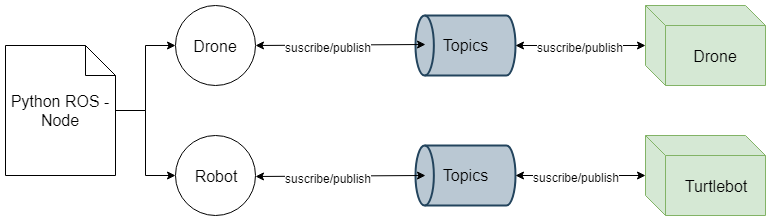
\includegraphics[scale=0.6]{img/s4r-diagrama-robot.png}
  	\caption{Esquema de comunicaciones ROS a través del nodo generado}
  	\label{fig:s4r-esquema}
\end{figure}

Apoyándonos en la figura 4.3, vamos a explicar la lógica implementada tras esta plantilla.\\

Como hemos planteado anteriormente, la traducción final se encapsula en una plantilla común a drones y Turtlebots, que no es ni más ni menos que el Nodo ROS que vamos a ejecutar. De cara a simplificar el código de salida generado por nuestra herramienta, hemos agrupado la lógica referida al procesado de comunicaciones ROS en dos librerías, una para Turtlebots y otra drones. De ahí a que en la figura 4.3 se hayan dividido estas dos partes. Entrando en detalle mostramos el código simplificado del nodo final generado.\\

\begin{lstlisting}[language=python,firstnumber=1]
#!/usr/bin/env python
# -*- coding: utf-8 -*-n
import ...
# Establece la subscripcion a topics ROS para drones
from drone import Drone 
# Establece la subscripcion a topics ROS para robots
from robot import Robot 
# Ejecucion del nodo  
def execute(robot):
    try:
    # Desde codigo, insertamos la traduccion obtenida aqui 
    // Scratch Code
    except KeyboardInterrupt:
        raise       
if __name__ == '__main__':
    # carga de configuraciones, topics ros a los que nos suscribimos, a traves de fichero yml
        cfg = config.load(open_path + filename)
        yml_file = yaml.load(stream) 
    for section in yml_file:
    # En el yml de configuracion se define si se trata de robot o drone.
        if section == 'drone':
        # Si es drone se inicia la clase que hace la subscripcion a todos los topics ROS
             robot = Drone(cfg)
        elif section == 'robot':
    	# De forma analoga si se trata de un robot sobre ruedas
             robot = Robot(cfg)
    execute(robot)

\end{lstlisting}

Como hemos comentado, la lógica referente a ROS se aplica a través de dos librerñias, \textit{drone} y \textit{robot}. Entrando en más detalle de estas librerías, vamos a ver como realiza la suscripción y publicación en los tópicos desde una de ellas, con fragmentos de códigos obtenidos de la aplicación.\\

\begin{lstlisting}[language=python,firstnumber=1]
import config
import rospy

class Robot():
    def __init__(self, cfg):
        # inicia nodo ROS Robot
        self.__node = rospy.init_node("robot", anonymous=True)
        # hacemos la subscripcion a los topics ROS
        topic = cfg.getProperty("robot.Pose3D.Topic")
        self.__pose3d_client = ListenerPose3d(topic)
        topic = cfg.getProperty("robot.Motors.Topic")
        self.__motors_client =  PublisherMotors(topic)
        
	def getPose3d():
		return self.__pose3d_client.getPose3d()
\end{lstlisting}

Describiendo el fragmento de código anterior y como se aprecia en el esquema de más arriba, nuestro nodo ROS en Python, a través del objeto Python \textit{Robot}, establece las comunicaciones ROS al iniciarse por primera vez. Esto se consigue con la carga de propiedades del fichero de configuración que se le pasa como argumento. Estas propiedades como hemos comentado anteriormente serán los tópicos a los que se conectará nuestro nodo. Se realizará la suscripción o publicación a cada tópico de manera individual. En este caso y observando el código,  usamos el objeto \textit{ListenerPose3d}, para conectarnos al tópico de el que obtendremos la información publicada por el sensor de odometría del robot, del mismo modo se hace con \textit{PublisherMotors} para el uso de los motores del robot.\\

En resumidas cuentas, al iniciarse el objeto Python, \textit{Robot} o \textit{Drone}, según se esté usando un tipo u otro, éste realiza la suscripción a todos los tópicos a través de la creación de un \textit{cliente} por cada una de estas suscripciones. Estos \textit{clientes} ya contienen métodos desde los que obtener mediante comunicaciones ROS, la información final tal y como la esperamos.\\

En el siguiente extracto de código se aprecia simplificado el detalle de una de los clientes que realizan la suscripción, y de los obtenemos información del robo, a través de mensajes ROS, publicados en un tópico.

\begin{lstlisting}[language=python,firstnumber=1]
# modulo python oficial ros
import rospy
# mensajes de comunicacion ROS para la lectura de odometria
from nav_msgs.msg import Odometry
class ListenerPose3d:
    def __init__(self, topic):
    	# Objeto Pose3d() contiene los datos devueltos por el sensor
        self.data = Pose3d() 
        # Al suscribirnos como argumento se introduce el topico,
        # el tipo de mensaje ROS que se lee del topico
# y una funcion de callback en la que recogemos las lecturas del topico
        self.sub = rospy.Subscriber(self.topic, Odometry, self.__callback)

    def __callback (self, odom):
        pose = odometry2Pose3D(odom)
        self.lock.acquire()
        self.data = pose
        self.lock.release()
        
    # metodo a traves del cual obtendremos la pose 3d    
    def getPose3d(self):
        self.lock.acquire()
        pose = self.data
        self.lock.release()
        return pose
\end{lstlisting}

Este mismo procedimiento hay que seguirlo para cada uno de los posibles tópicos ROS que necesite nuestra aplicación, por ejemplo, uno para dar velocidad a los distintos motores, otro para el sensor láser, cámaras incrustadas en el robot etcétera.\\

Con todo esto se puede apreciar la complejidad de la que evadimos al usuario, siendo para él, un simple ejecutable o nodo, completamente operativo, generado a través de nuestra aplicación. Una vez lanzado el nodo habremos sido capaces de aplicar una lógica programada en Scratch sobre un robot en un entorno simulado. 


\section{Traducción de bloques}
Una vez entendido el funcionamiento de la plantilla encargada de toda la lógica de funcionamiento sobre comunicaciones ROS, y volviendo a la figura 4.2, vamos a especificar como se lleva a cabo la traducción del programa Scratch y las mejoras que hemos llevado a cabo en este proceso.\\

Esta labor de traducción la realizamos a través del uso de la bibliotea Kurt, vamos a estudiar más a fondo como trabaja la esta biblioteca y cómo nos ha ayudado en la traducción de bloques.\\

Kurt es una biblioteca de Python que permite la manipulación compleja de proyectos Scratch (archivos .sb o .sb2) a través de simples comandos de Python. Incluye un decompilador, que permite que un proyecto se cargue en un conjunto de objetos de Python, y un compilador que permite el empaquetamiento de un conjunto de \textit{scripts} de imágenes / texto en proyectos Scratch.\\

En este proyecto se ha utilizado una versión\footnote{\url{https://pypi.org/project/jderobot-kurt/}} mejorada de esta biblioteca, con ciertas adaptaciones para el tratamiento de extensiones externas como la nuestra. Kurt define los bloques usados por Scratch como objetos JSON, en esta nueva versión se agrega un fichero con la configuración de nuestros bloques como objetos JSON. De esta forma se agrega la capacidad de obtener la información de los bloques de nuestra extensión.\\

La clase principal de kurt almacena el contenido de un archivo de proyecto Scratch. Los contenidos incluyen variables globales y listas, el escenario y los \textit{sprites}, cada uno con sus propios \textit{scripts}, sonidos, variables y listas.\\

Una vez obtenido el contenido de un proyecto Scratch en un objeto Python, con el siguiente fragmento de código somos capaces de obtener el \textit{strings} representativo de cada bloque.\\

\begin{lstlisting}[language=python,firstnumber=1]
# load the scratch project
p = kurt.Project.load(open_path + sys.argv[1])

# show the blocks included
for scriptable in p.sprites + [p.stage]:
	for script in scriptable.scripts:
		# exclude definition scripts
		if "define" not in script.blocks[0].stringify():
			s = script
print("Stringify:")
sentences = []
for b in s.blocks:
	print(b.stringify())
\end{lstlisting}

Una vez tenemos la lista de los \textit{strings} equivalentes a los bloques del proyecto Scratch, hay que realizar una tarea de transformación de estas a código Python.\\

En este trabajo se modifica de forma notable la forma en la que se realizaba de forma inicial esta traducción, agregando una gran cantidad de bloques soportados y añadiendo un grado de recursividad que permite la traducción de bloques anidados. El soporte de bloques anidados nos permite realizar acciones de mayor complejidad dentro del entorno Scratch, como pueden ser bucles en los que se definen flujos condicionales complejos.\\

En la traducción nos apoyamos de unos diccionarios Python en los que mapeamos el string equivalente al bloque Scratch con el equivalente Python que queremos sustituir, esto nos lleva al último punto de nuestro desarrollo. Para ciertos bloques de Scratch existe una traducción directa a un comando Python como ya hemos visto antes. Mientras que para los bloques robóticos definidos por nuestra extensión debemos de crear un método específico que contenga toda la lógica a implementar como hemos visto anteriormente en la descripción de nuestros bloques.\\

\section{Desarrollo de bloques}
\label{sec:desarrollo-de-bloques}

Una de las aportaciones de este trabajo a la herramienta ha sido la refactorización de bloques ya existentes y la agregación de nuevos bloques funcionales. En la programación visual entendemos por bloque a cada componente visual que contiene una lógica específica, con la agrupación de bloques podemos conseguir un flujo de programación complejo. En primer lugar vamos a describir como hemos agregado estos nuevos bloques a Scratch, siguiendo con su definición e implementación.

\subsection{Extensión de Scratch}

Para la agregación de nuevos bloques, Scratch facilita el uso de extensiones externas, estas  extensiones definen mediante el uso de ficheros .s2e compuesto por una serie de objetos JSON. Este tipo de ficheros se creó para la comunicación mediante HTTP de bloques con aplicaciones auxiliares, por ejemplo algún tipo de hardware. Nosotros no vamos a utilizar esta funcionalidad, únicamente nos ayudamos de este documento .s2e para definir nuestra extensión y pueda ser usada desde el IDE offline de scratch.\\

En este documento se define un objeto JSON, el cual será la definición de la extensión, en el que se incluye el nombre de la extensión, un puerto usado para la comunicación de componentes externos en caso de ser necesario y una lista de bloques de Scratch. \\

A continuación se define un ejemplo de una extensión para Scratch. 
\begin{lstlisting}[language=json,firstnumber=1]
{ 
  "extensionName": "Extension Example",
  "extensionPort": 12345,
  "blockSpecs": [
    [" ", "beep", "playBeep"],
	[" ", "set beep volume to %n", "setVolume", 5],
	["r", "beep volume", "volume"],
  ]
}
\end{lstlisting}

El campo ``blockSpecs'' describe los bloques de extensión que aparecerán en el apartado ``Más bloques'' en la aplicación de Scratch.
En en este caso, hay tres bloques:
\begin{itemize}
\item Un bloque de comandos que reproduce un pitido.
\item Un bloque de comando que
establece el volumen del pitido.
\item Un bloque que devuelve un valor, que informa del volumen de un pitido.
\end{itemize}

Cada bloque se describe mediante una matriz con los siguientes campos:
\begin{itemize}
\item \textbf{Tipo de bloque}:

\begin{itemize}
\item ' ' - bloque de comandos
\item 'w' - bloque de comandos que esperan
\item 'r' - bloque que retorna un valor
\item 'b' - bloque que retorna un booleano 
\end{itemize}
\item \textbf{Formato de bloque}:

El formato de bloque es una cadena que describe las etiquetas y ranuras de parámetros que aparecen en el bloque.
Las ranuras de parámetros están indicadas por una palabra que comienza con '\%' y puede ser una de:
\begin{itemize}
\item \%n -  parámetro de número 
\item \%s - parámetro de cadena 
\item \%b - parámetro booleano
\end{itemize}
\item \textbf{Operación o nombre de variable remota}:

El campo de operación en una especificación de bloque se usa de dos maneras. Para bloques de comandos, se envía a la aplicación auxiliar, junto con cualquier valor de parámetro, para invocar una operación. O para retornar bloques, es el nombre de una variable de sensor. Los valores de la variable del sensor se guardan en un diccionario. La ejecución de un bloque simplemente devuelve el valor reportado más recientemente para esa variable de sensor.
\item \textbf{Parámetros predeterminados}:

Se pueden añadir cero o más valores de parámetros predeterminados

\item \textbf{Menús desplegables}:

Los bloques que definimos pueden hacer uso de parámetros de menú, los cuales definiremos de dos formas:
\begin{itemize}
\item \%m.menuName - parámetro de menú (no editable), proporciona un sencillo espacio para los parámetros del menú desplegable.
\item \%d.menuName - parámetro de número editable con menú, proporciona una ranura de parámetro numérico con un menú auxiliar.
\end{itemize}
\end{itemize}

Con todo esto podemos entender la definición de alguno de nuestros bloques como podemos en el siguiente extracto de código, en el que se ve la definición de algunos de nuestros bloques.
\begin{nobreak} 
\begin{lstlisting}[language=json,firstnumber=1]
{
  "extensionName": "Scratch4Robots",
  "extensionPort": 12345, 
  "blockSpecs": [
    ["", "stop robot-drone", "stop"],         
    ["", "move robot %m.robotDirections speed %n", "robot/move/speed", "forward", 1],
    ["r", "color detection %m.color", "camera/all","red"],
    ["r", "frontal laser distance", "laser/frontal"],
  ],
  "menus": {
    "robotDirections": ["forward", "back"],         
    "color": ["red", "blue"]
  }
}

\end{lstlisting}
\end{nobreak} 

\subsection{Bloques genéricos}
Antes de comenzar con los bloques propios a nuestra extensión vamos a necesitar una serie de bloques genéricos que nos ayuden a realizar lógica básica de programación como pueden ser operadores matemáticos, operadores lógicos y sentencias básicas de programación. Scratch ya nos ofrece estos bloques por definición, por lo que no hará falta agregarlos a nuestra extensión específica, solamente nos encargaremos de su posterior traducción a código Python.\\

A continuación mostramos todos los bloques genéricos de los que podemos hacer uso desde la herramienta Scratch4Robots, ya que hemos implementado su traducción a Python.

\begin{itemize}
\item \textbf{Bloques de operadores matemáticos}:

Bloques fundamentales de cara a realizar una lógica posterior con los datos obtenidos desde los sensores de nuestros robots, estos bloques son una de las mejoras ofrecidas por este trabajo.
\begin{figure}[H]
    	\centering
    	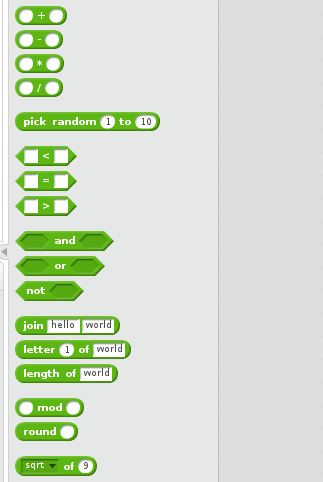
\includegraphics[scale=0.60]{img/bloques-mat.png}
     	\caption{Bloques matemáticos y lógicos}
  	\label{fig:mat}
\end{figure}

	\begin{itemize}

    \item \textbf{sqrt of ()}: Realiza la operación raíz cuadrada de un número dado
    \item \textbf{sin of ()}: Realiza la operación seno de un número dado
    \item \textbf{cos of ()}: Realiza la operación coseno de un número dado
    \item \textbf{tan of ()}: Realiza la operación tangente de un número dado
    \item \textbf{asin of ()}: Realiza la operación arcoseno de un número dado
    \item \textbf{acos of ()}: Realiza la operación arcocoseno de un número dado
    \item \textbf{atan of()}: Realiza la operación arcotangente de un número dado
    \item \textbf{log of ()}: Realiza la operación logaritmo de un número dado
    \item \textbf{ln of ()}: Realiza la operación logaritmo neperiano de un número dado
    \item \textbf{abs of ()}: Devuelve el valor absoluto de un número
    \item \textbf{mod of ()}: Devuelve el módulo de un número dado
    \end{itemize}

\item \textbf{Bloques de operadores lógicos}:
Permiten construir expresiones lógicas, se obtiene como resultado booleanos.
\begin{itemize}

 \item \textbf{And}: Operador de conjunción.
 \item \textbf{Or}: Operador de disyunción.
 \item \textbf{NOT}: Operador de negación.
 \item \textbf{Mayor que y Menor que}: Operadores de comparación numérica.
\end{itemize}

\item \textbf{Bloques de control}:

Estructuras de control básicas de programación.

\begin{figure}[H]
    	\centering
    	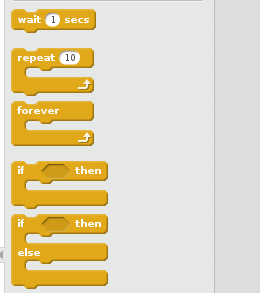
\includegraphics[scale=0.60]{img/bloques-control.png}
     	\caption{Bloques de control}
  	\label{fig:control}
\end{figure}
\begin{itemize}
\item \textbf{Wait () secs}: Pausa la ejecución el tiempo especificado, equivalente a la sentencia \textit{time.sleep()} de Python.
\item \textbf{Forever}: Bucle infinito, equivalente a \textit{while(True)} en lenguaje Python.
\item \textbf{If () then}: Comprueba la condición para que si la condición es verdadera, los bloques dentro de ella se ejecuten.
\item \textbf{If () Then, Else}: Comprueba la condición para que si la condición es verdadera, los bloques dentro de la primera condición se activen y si la condición es falsa, los bloques dentro de la segunda condición se activarán.
\item \textbf{Repeat ()}: Un ciclo que repite la cantidad de veces especificada, sería la equivalencia al bucle \textit{for} en Python.
\end{itemize}
\item \textbf{Otros}
\begin{itemize}

\item \textbf{say ()}: Imprime lo que le añadas como argumento, equivalente a \textit{print}.
\item \textbf{Set () to ()}: Utilizado para dar valor a una variable en concreto.
\end{itemize}

\item \textbf{Bloques de listas}:

Esta serie de bloques desarrollados en esta versión han sido de gran ayuda a la hora de la refactorización y creación de otros bloques de mayor complejidad.

\begin{figure}[H]
     	\centering
     	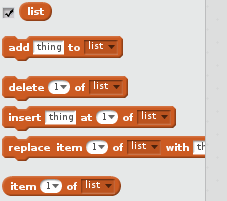
\includegraphics[scale=0.60]{img/bloques-listas.png}
     	\caption{Bloques de listas}
  	\label{fig:listas}
\end{figure}

\begin{itemize}
\item \textbf{Insert () at () of ()}: Inserta elemento en la posición seleccionada de la lista indicada.
\item \textbf{Item () of ()}: Devuelve el elemento almacenado en la posición indicada de la lista.
\item \textbf{Add () to ()}: Inserta en la lista un elemento.
\item \textbf{Delete () of ()}: Elimina el elemento en una posición determinada de la lista.
\end{itemize}
\end{itemize}

\subsection{Bloques para drones}
Estos bloques ya pertenecen a la extensión creada para la herramienta.
En este trabajo se ha realizado una refactorización completa de todos los bloques referentes a drones y la agregación de nuevos bloques. 

Cabe destacar de estos bloques que una vez traducidos al nodo final, que se consigue implementar el funcionamiento de drones bajo comunicación ROS, ésto es algo elaborado completamente en este trabajo.\\

Para ello nos apoyamos en MAVROS\footnote{\url{http://wiki.ros.org/mavros}}, puente oficial entre nodos ROS y Mavlink\footnote{\url{https://github.com/mavlink}}, el protocolo de comunicación estándar para drones.

\begin{itemize}
\item \textbf{Bloques perceptivos}:
Nos permiten obtener información de sensores incorporados en el drone.
	\begin{itemize}
	\item \textbf{Get pose3D}: Obtiene el valor de la posición 3D del robot.
		\begin{figure}[H]
     		\centering
     		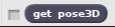
\includegraphics[scale=1.2]{img/block-pose.png}
     		\caption{bloque que retorna la posición del robot}
  		\label{fig:listas}
		\end{figure}
Simplificando la totalidad del código, la función Python en la que quedaría traducida sería \textit{getPose3d}, como se muestra:\\

\begin{lstlisting}[language=python,firstnumber=1]
    def getPose3d(self):
    	# client_pose3d se trata del cliente que hace la comunicacion ROS
        return client_pose3d.getPose3d
\end{lstlisting}
	\item \textbf{Color detection}: Nuevo componente añadido en esta versión, que haciendo uso de una cámara en el robot, detecta objetos de un determinado color, introducido como argumento, devolviendo una lista que contendrá las posiciones en los ejes x e y, además del tamaño del objeto, en la imagen capturada por la cámara.\\
	\begin{figure}[H]
     		\centering
     		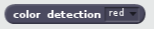
\includegraphics[scale=1.2]{img/block-color.png}
     		\caption{bloque que detecta objetos de un determinado color}
  		\label{fig:listas}
  				\end{figure}
  				
 Usando la biblioteca OpenCV de Python y con técnicas de análisis computacional de imágenes, de una simple imagen somos capaces de obtener su posición en la imagen y su tamaño:\\
 
 \begin{lstlisting}[language=python,firstnumber=1]
    def detect_object(self, color):
        # define the lower and upper boundaries of the basic colors
        color_range = __get_color_range(color)
        # get image type from camera ROS client
        image = self.__camera_client.getImage()
        # apply color filters to the image
        filtered_image = cv2.inRange(image.data, color_range[0], color_range[1])
        rgb = cv2.cvtColor(image.data, cv2.COLOR_BGR2RGB)
        # Apply threshold to the masked image
        ret,thresh = cv2.threshold(filtered_image,127,255,0)
        im,contours,hierarchy = cv2.findContours(thresh,cv2.RETR_TREE,cv2.CHAIN_APPROX_SIMPLE)
        # Find the index of the largest contour
        for c in contours:
            if c.any != 0:
                areas = [cv2.contourArea(c) for c in contours]
                max_index = np.argmax(areas)
                cnt=contours[max_index]
                if max(areas) > 0.0:
                    x,y,w,h = cv2.boundingRect(cnt)
                    x_position = (w/2)+x
                    y_position = (h/2)+y
                    size = w*h
        return size, x_position, y_position
\end{lstlisting}


	\end{itemize}
\item \textbf{Bloques de movimiento}
	\begin{itemize}
	\item \textbf{Stop robot-drone}: Pone a su valor inicial todas las velocidades del robot.\\
	\begin{figure}[H]
     		\centering
     		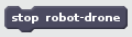
\includegraphics[scale=1.2]{img/block-stop.png}
     		\caption{bloque stop-robot}
  		\label{fig:listas}
  				\end{figure}
Con el código que se ejecutará tras su traducción:\\

 \begin{lstlisting}[language=python,firstnumber=1]
    def stop_robot(self):
        self.client__vel.sendVelocities(0,0,0,0,0,0)
        time.sleep(1)

\end{lstlisting}

	\item \textbf{Drone take off}: Hace que el drone despegue.\\
	\begin{figure}[H]
     		\centering
     		
\includegraphics[scale=1.2]{img/block-takeoff.png}
     		\caption{bloque que realiza el despegue del drone}
  		\label{fig:listas}
  				\end{figure}
  				
Mediante el armado del drone y el envío de una velocidad ascendente conseguimos su despegue:\\

 \begin{lstlisting}[language=python,firstnumber=1]
    def takeoff(self):
    	# arming realiza el encendido del robot
        self.client_extra.arming()
        self.client_vel.sendVelocities(0,0,2,0,0,0)
        time.sleep(1)
        self.client_vel.sendVelocities(0,0,0,0,0,0)
\end{lstlisting}

	\item \textbf{Drone land}: Realiza un aterrizaje controlado del drone.\\
	\begin{figure}[H]
     		\centering
     		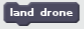
\includegraphics[scale=1.2]{img/block-land.png}
     		\caption{bloque que realiza el aterrizaje del drone}
  		\label{fig:listas}
  				\end{figure}
Para realizar el aterrizaje del drone a través de ROS, tiene su propio tópico al cual se le envía una llamada con argumentos cero, como se puede observar:\\

 \begin{lstlisting}[language=python,firstnumber=1]
    def land(self):
        self.lock.acquire()
        self.land_client.call(0,0,0,0,0)
        self.lock.release()
\end{lstlisting}
	

	\item \textbf{Move drone}: Bloque que tras la refactorización admite una lista con las velocidades del drone en los diferentes ejes (velocidad en el eje x, velocidad en el eje z, velocidad yaw), pare realizar giros se debe combinar la velocidad en el eje x con la velocidad de rotación en yaw.\\
	\begin{figure}[H]
     		\centering
     		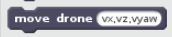
\includegraphics[scale=1.2]{img/block-move-drone.png}
     		\caption{bloque que realiza el despegue del drone}
  		\label{fig:listas}
  	\end{figure}
  	
Lo que se traduce a python con la siguiente función:\\
  	
\begin{lstlisting}[language=python,firstnumber=1]
 def move_vector(self, velocities):
    # cliente que realiza la suscripcion al topico que recibe la pose
    pose = self.client__pose3d.getPose3d()
    yaw = pose.yaw
    vx = velocities[0]
    vz = velocities[1]
    az = velocities[2]
    vxt = vx*math.cos(yaw)
    # cliente que realiza la suscripcion al topico que publica velocidades
    self.client__vel.sendVelocities(vxt,0,vz,0,0,az)
\end{lstlisting}
	
	\end{itemize}
\end{itemize}



\subsection{Bloques para Turtlebots}
\begin{itemize}
\item \textbf{Bloques perceptivos}
	\begin{itemize}
	\item \textbf{Pose3D} :Obtiene el valor de la posición 3D del robot.
		\begin{figure}[H]
     		\centering
     		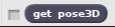
\includegraphics[scale=1.2]{img/block-pose.png}
     		\caption{bloque pose del robot}
  		\label{fig:listas}
  	\end{figure}
Se traduce de forma equivalente a su homólogo para drones, la única diferencia es el tópico desde el que recibe la información.\\
 
	\item \textbf{Color detection}: Bloque homólogo al del drone, dado un color nos devuelve su posición en la imagen, y su tamaño.
		\begin{figure}[H]
     		\centering
     		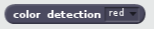
\includegraphics[scale=1.2]{img/block-color.png}
     		\caption{bloque que detecta colores en una imagen}
  		\label{fig:listas}
  	\end{figure}
Se trata del mismo bloque perceptivo ya definido para drones.\\

\item \textbf{Frontal distance}: Obtiene la medida promedio de los datos del láser frontal. 
		\begin{figure}[H]
     		\centering
     		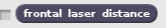
\includegraphics[scale=1.2]{img/block-laser.png}
     		\caption{bloque que devuelve datos de un laser}
  		\label{fig:listas}
  	\end{figure}
Se traduce al siguiente método Python:\\

\begin{lstlisting}[language=python,firstnumber=1]
def get_laser_distance(self):
        # get laser values from ROS client
        laser = self.__laser_client.getLaserData()
        l = [x for x in laser.values if str(x) != 'nan' and x < 10]
        try:
            avg = sum(l) / len(l)
        except ZeroDivisionError:
            avg = 0
        return avg
\end{lstlisting}

	\end{itemize}
\item \textbf{Bloques de movimiento}
	\begin{itemize}

	\item \textbf{robot move ()}: Admite como parámetro una lista con las velocidades en el eje x y eje z.
		\begin{figure}[H]
     		\centering
     		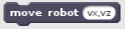
\includegraphics[scale=1.2]{img/block-move-robot.png}
     		\caption{bloque de movimiento para robots}
  		\label{fig:listas}
  	\end{figure}
  	
Con su traducción:\\

\begin{lstlisting}[language=python,firstnumber=1]
    def move_vector(self, velocities):
        vx = float(velocities[0])
        vz = float(velocities[1])
        print "velocities:",vx,vz
        self.__reset()
        self.__vel.vx = vx
        self.__vel.vz = vz
        if vz>0:
            self.turn("left",vz)
        if vz<0:
            self.turn("right",vz)
        self.__publish(self.__vel)
\end{lstlisting}

	\item \textbf{robot turn ()}: Permite la rotación sobre el propio eje del robot.
	\begin{figure}[H]
     		\centering
     		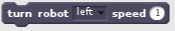
\includegraphics[scale=1.2]{img/block-turn.png}
     		\caption{bloque que realiza el giro del robot}
  		\label{fig:listas}
  	\end{figure}
  	
Con su traducción Python:\\

\begin{lstlisting}[language=python,firstnumber=1]
    def turn(self, direction, vel):
        self.__vel.az = vel
        # set different direction
        if direction == "right":
            self.__vel.az = -self.__vel.az
        # publish movement
        self.__publish(self.__vel)
\end{lstlisting}
	\end{itemize}
\end{itemize}

Con esto se definen los bloques pertenecientes a nuestra extensión, de la forma en que Scratch los muestra y la traducción de cada uno de ellos llevada, de una forma simplificada. Se aprecia que se trata de robots sofisticados, con cierta complejidad. La cual hacemos transparente para el usuario, simplificando toda la lógica que existe tras cada robot, en simples e intuitivos bloques gráficos.

En este trabajo hemos refactorizado la totalidad de la lógica tras los bloques robóticos, dándole una mayor coherencia a todos ellos. Además de crear lógica completamente nueva para ciertos bloques agregados en esta versión. Cabe destacar el bloque referente a la detección de objetos de un cierto color.\\






